\documentclass[a4paper, 11pt]{article}
\usepackage{comment}
\usepackage{lipsum}
\usepackage{fullpage}
\usepackage[utf8]{inputenc}
\usepackage[T1]{fontenc}
\usepackage{libertine}
\usepackage{libertinust1math}
\usepackage{graphicx}
\usepackage{svg}


\begin{document}

\noindent
\large\textbf{Algorithmen und Datenstrukturen} \hfill \textbf{Christoph Stach (555912)} \\
\normalsize Aufgabe 3: Stack \hfill Tom Buhrtz \\

\section*{Aufgabenblatt 3 - 2}

\subsection*{Adjazenzmatrix}
\begin{tabular}{ |c|c|c|c|c|c|c| }
\hline
 & \textbf{A} & \textbf{B} & \textbf{C} & \textbf{D} & \textbf{E} & \textbf{F} \\
\hline
\textbf{A} & 0 & 1 & 1 & 1 & 1 & 1 \\
\hline
\textbf{B} & 1 & 0 & 0 & 0 & 0 & 0 \\
\hline
\textbf{C} & 1 & 0 & 0 & 0 & 0 & 0 \\
\hline
\textbf{D} & 1 & 0 & 0 & 0 & 0 & 0 \\
\hline
\textbf{E} & 1 & 0 & 0 & 0 & 0 & 0 \\
\hline
\textbf{F} & 1 & 0 & 0 & 0 & 0 & 0 \\
\hline
\end{tabular}

\subsection*{Adjazenzliste}
\begin{tabular}{ |c|c|c|c|c|c| }
\hline
\textbf{A} & \textbf{B} & \textbf{C} & \textbf{D} & \textbf{E} & \textbf{F} \\
\hline
\hline
B & A & A & A & A & A \\
\hline
C & & & & & \\
\hline
D & & & & & \\
\hline
E & & & & & \\
\hline
F & & & & & \\
\hline
\end{tabular}


\subsection*{Mathematische Darstellung}
\( G = \{ V , X \} \) \\
\( V = \{ A , B , C , D , E , F \} \)  \\
\( \vec X = \{ (A,B) , (A,C) , (A,D) , (A,E) , (A,F) , (B,A) , (C,A) , (D,A) , (E,A) , (F,A) \} \)

\pagebreak

\section*{Aufgabenblatt 3 - 3}

\subsection*{Adjazenzmatrix}
\begin{tabular}{ |c|c|c|c|c|c|c| }
\hline
 & \textbf{A} & \textbf{B} & \textbf{C} & \textbf{D} & \textbf{E} & \textbf{F} \\
\hline
\textbf{A} & 0 & 1 & 1 & 1 & 1 & 1 \\
\hline
\textbf{B} & 0 & 0 & 0 & 0 & 0 & 0 \\
\hline
\textbf{C} & 0 & 0 & 0 & 0 & 0 & 0 \\
\hline
\textbf{D} & 0 & 0 & 0 & 0 & 0 & 0 \\
\hline
\textbf{E} & 0 & 0 & 0 & 0 & 0 & 0 \\
\hline
\textbf{F} & 1 & 0 & 0 & 0 & 0 & 0 \\
\hline
\end{tabular}

\subsection*{Graph}
\includegraphics[width=0.5\linewidth]{img/pdf/Aufgabe_3-3}


\subsection*{Mathematische Darstellung}
\( G = \{ V , X \} \) \\
\( V = \{ A , B , C , D , E , F \} \)  \\
\( \vec X = \{ (A,B) , (A,C) , (A,D) , (A,E) , (A,F) , (F,A) \} \)

\pagebreak

\section*{Aufgabenblatt 3 - 4}

\subsection*{Adjazenzliste}
\begin{tabular}{ |c|c|c|c|c|c| }
\hline
\textbf{1} & \textbf{2} & \textbf{3} & \textbf{4} & \textbf{5} & \textbf{6} \\
\hline
\hline
2 | 5 & & & & & \\
\hline
3 | 3 & & & & & \\
\hline
4 | 11 & & & & & \\
\hline
5 | 1 & & & & & \\
\hline
6 | 9 & & & & & \\
\hline
\end{tabular}

\subsection*{Graph}
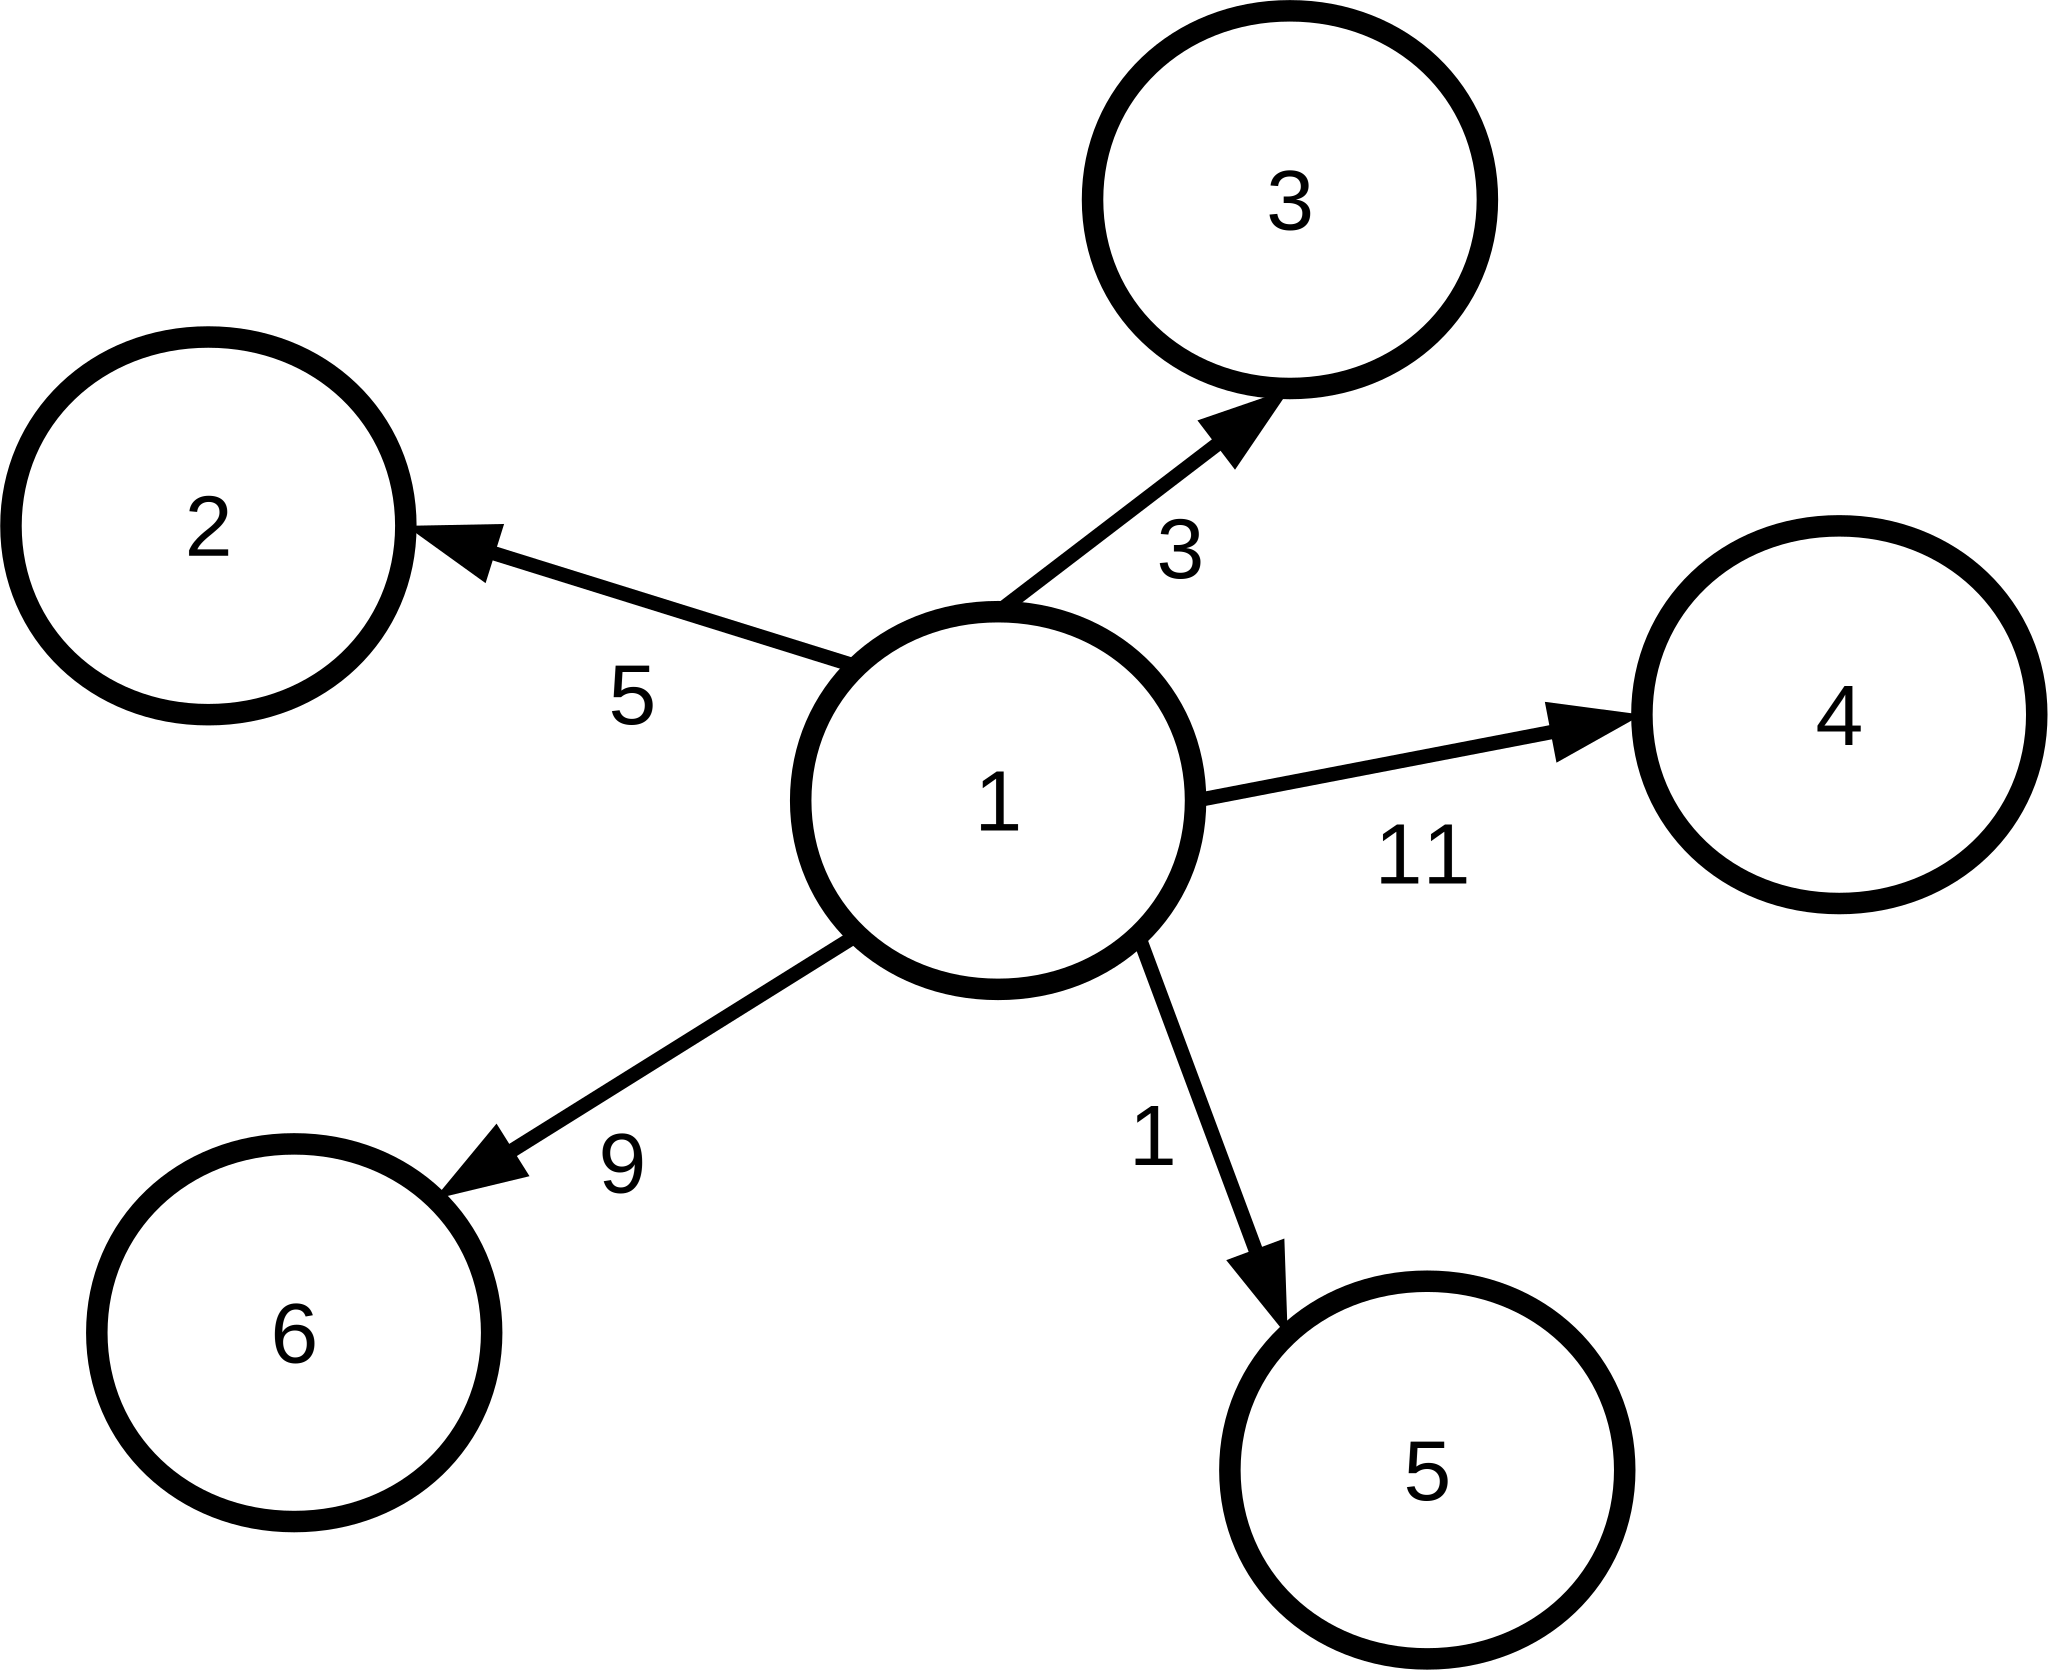
\includegraphics[width=0.5\linewidth]{img/pdf/Aufgabe_3-4}

\subsection*{Mathematische Darstellung}
\( G = \{ V , X \} \) \\
\( V = \{ 1 , 2 , 3 , 4 , 5 , 6 \} \)  \\
\( \vec X = \{ (1,2,5) , (1,3,3) , (1,4,11) , (1,5,1) , (1,6,9) \} \)



%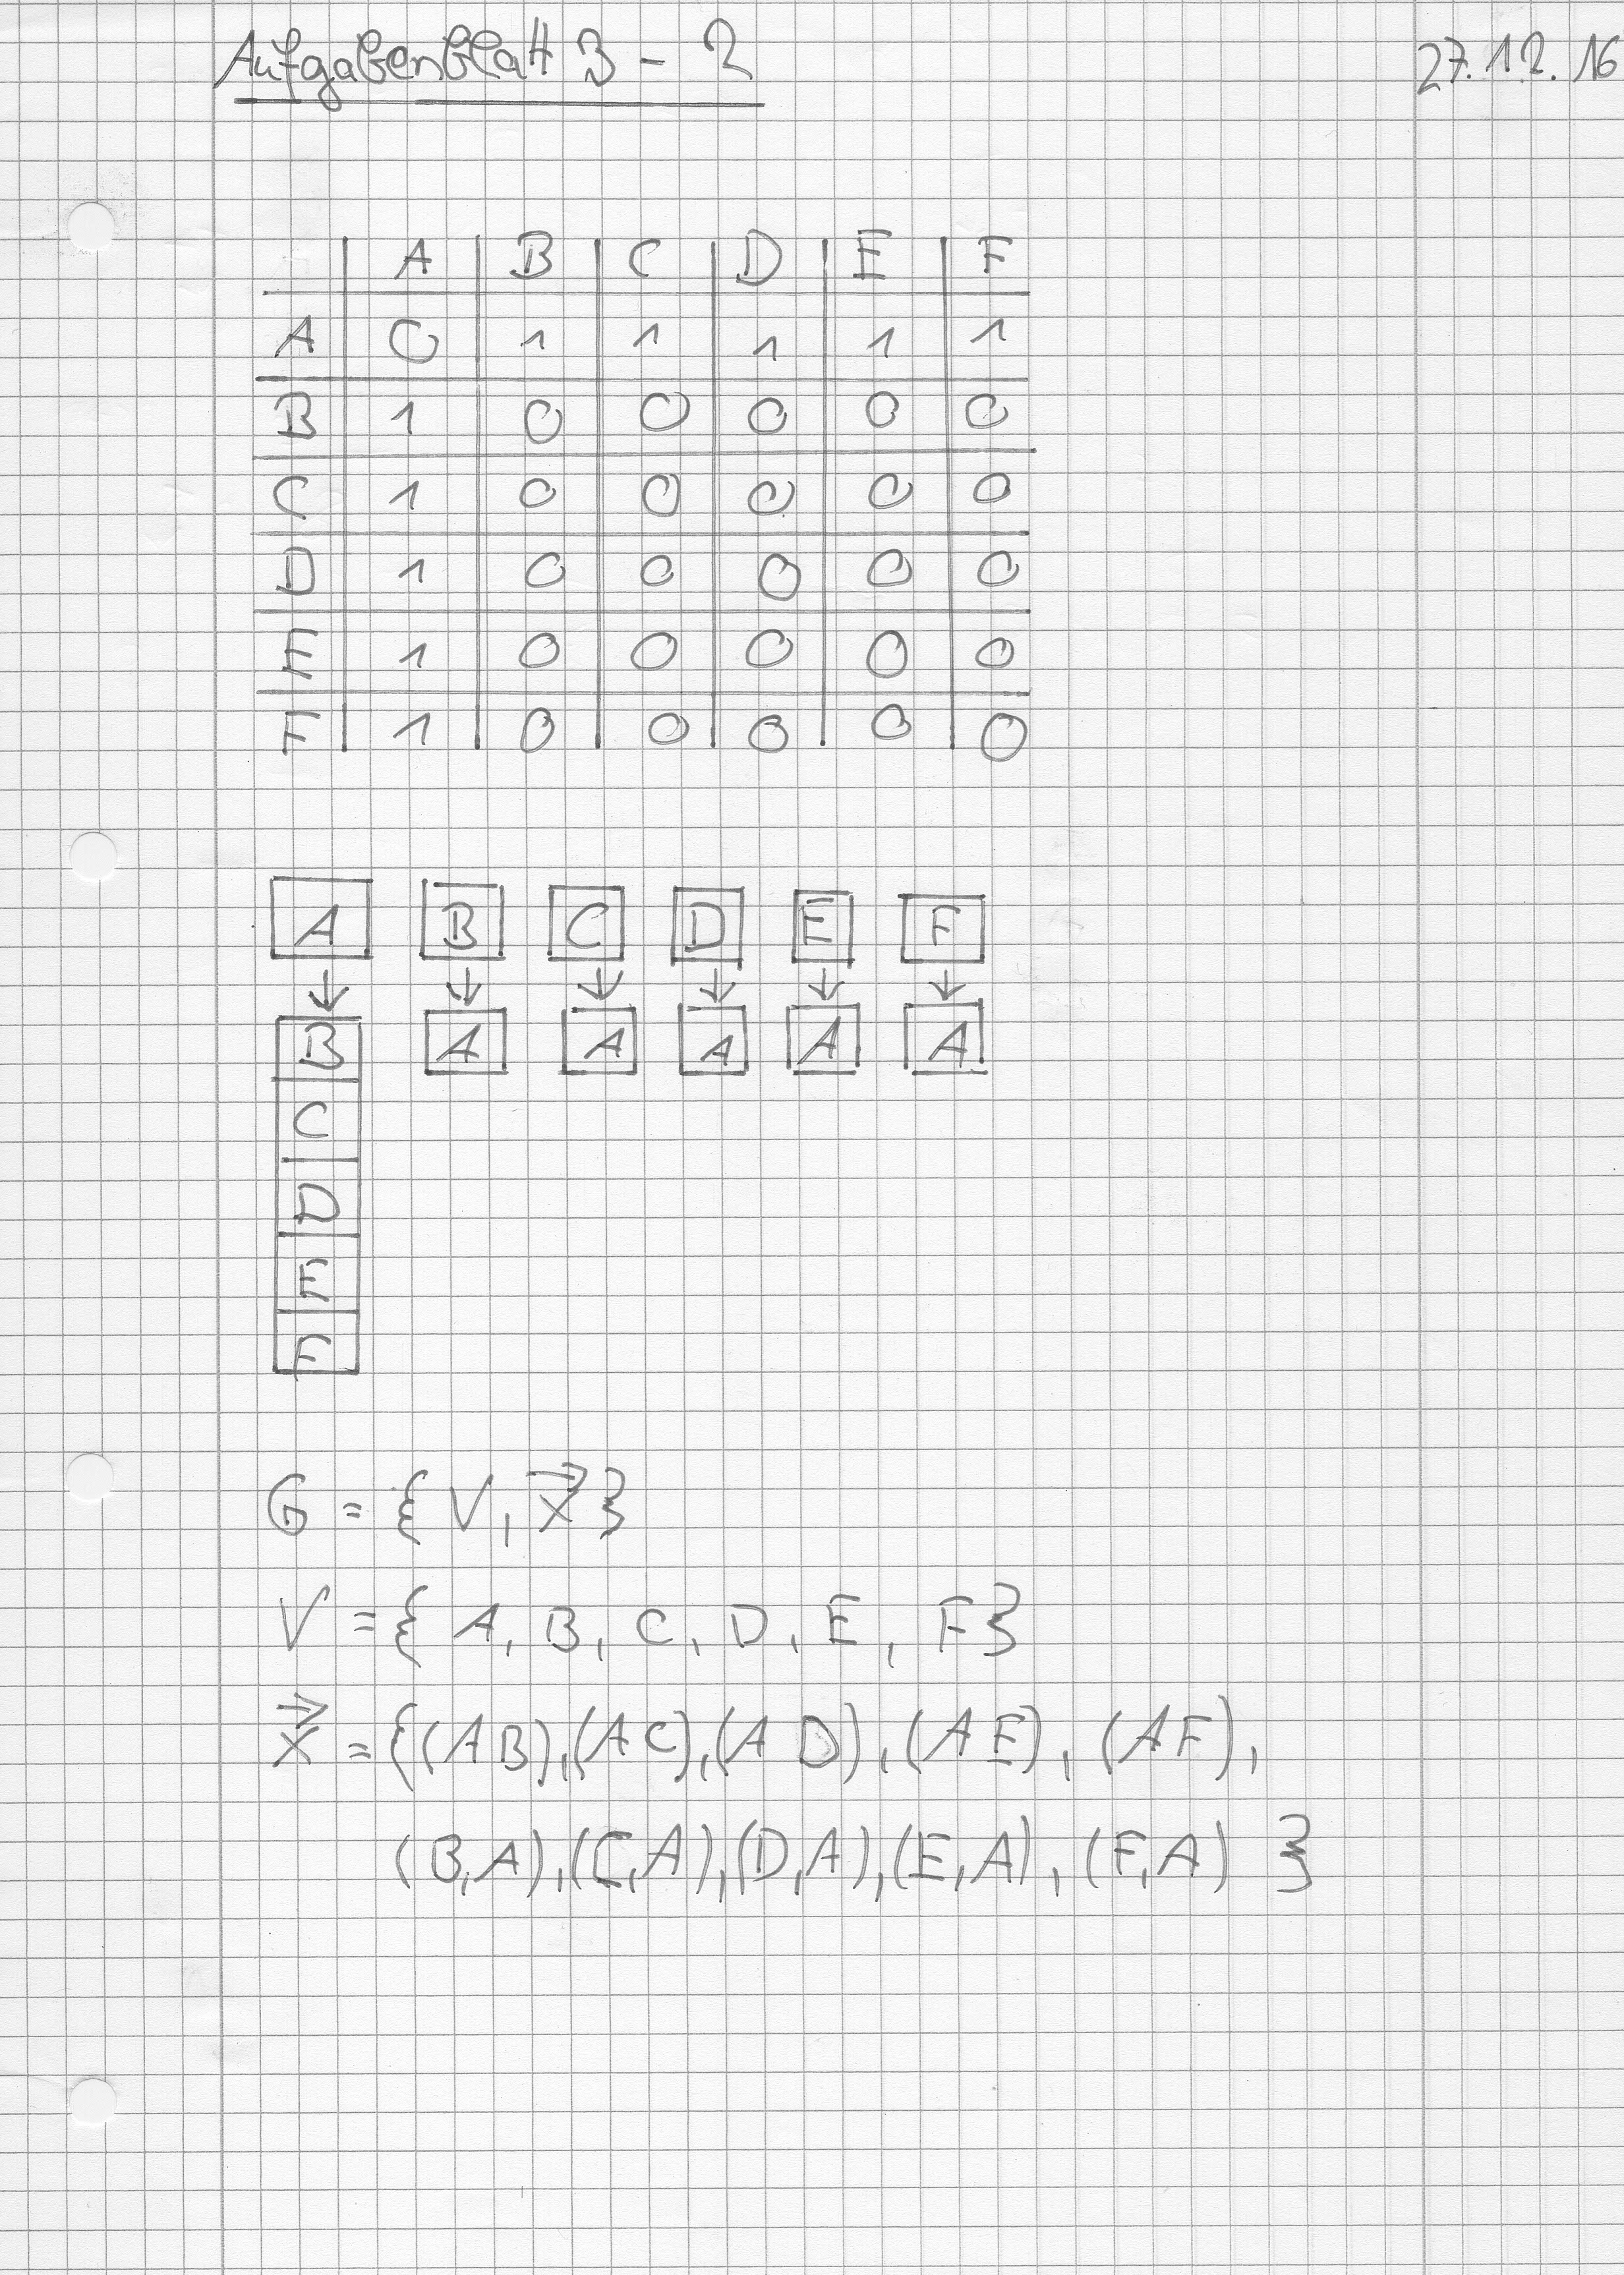
\includegraphics[width=15cm]{img-1}
%\pagebreak

%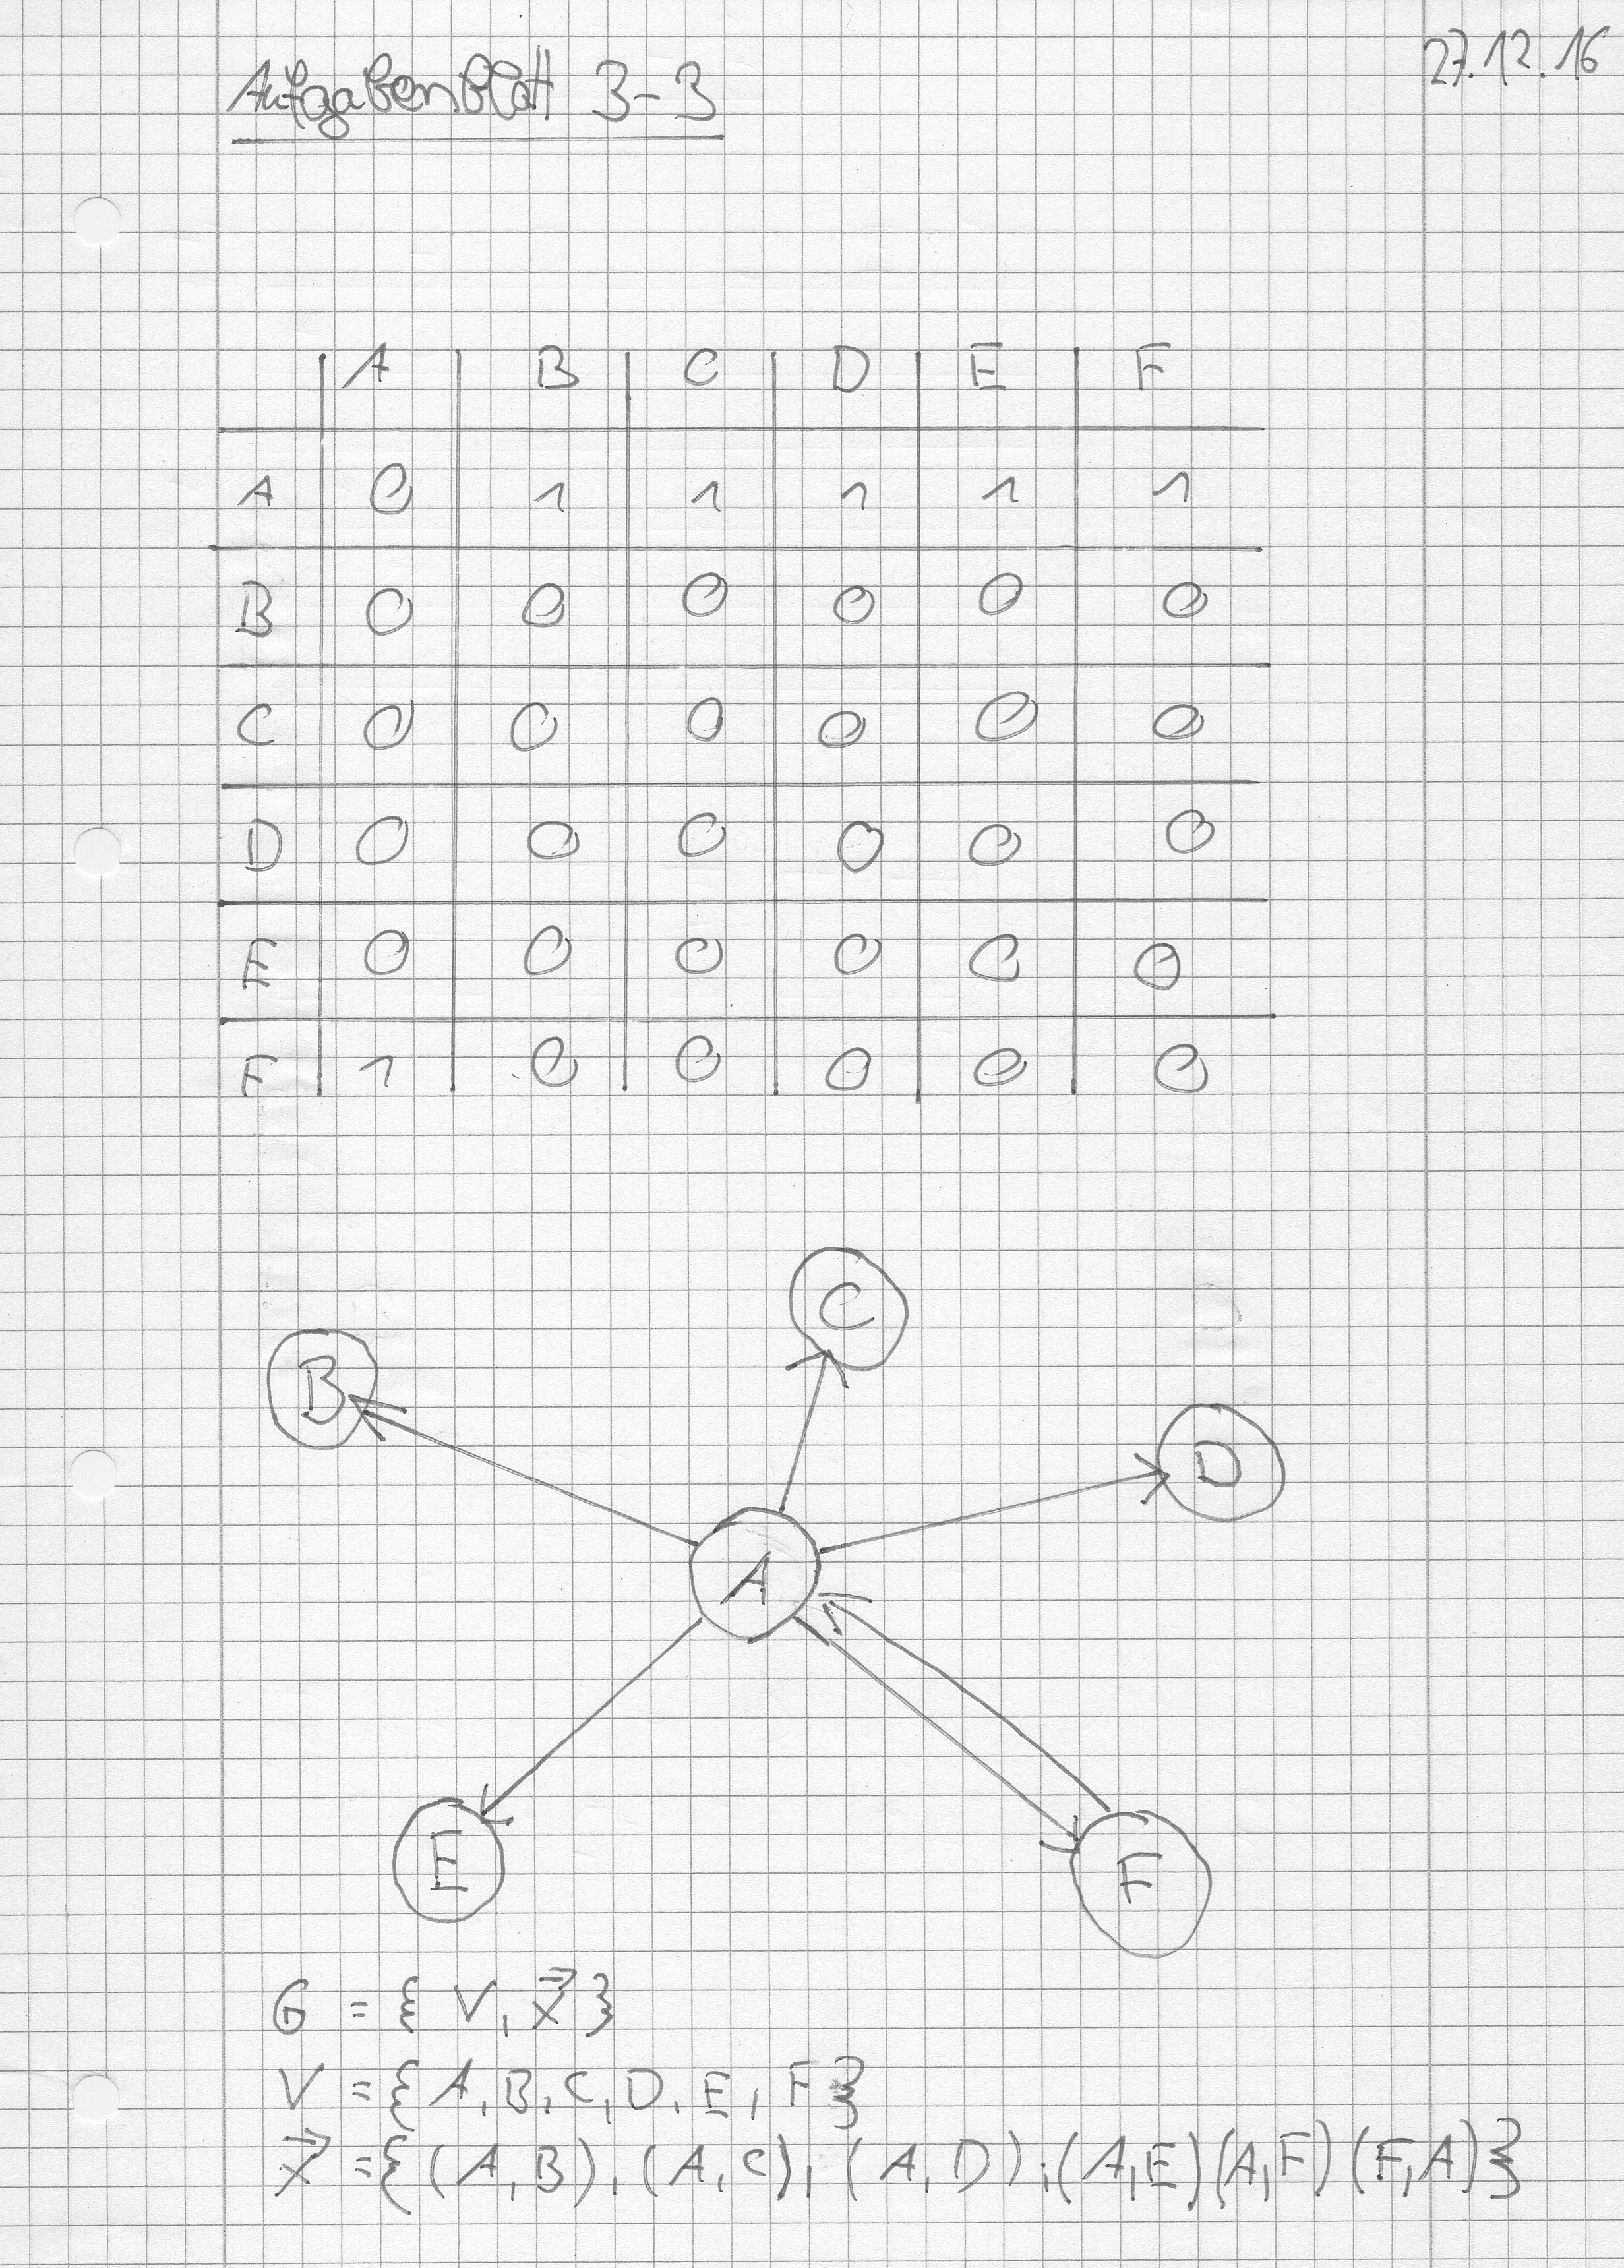
\includegraphics[width=15cm]{img-2}
%\pagebreak

%\includegraphics[width=15cm]{img-3}
%\pagebreak


\end{document}
